\chapter{Results \& Discussions}



This chapter presents algorithmic comparisons, infrastructure design decisions, the measured end-to-end latency budget, and screenshots of the deployed AWS-hosted system in operation.

\section{Algorithm Comparison: SVD + RANSAC vs.\ Alternatives}

Table~\ref{tab:summary_7} compares the chosen calibration approach against the principal alternatives considered during design.

\begin{table}[H]
\caption{Comparison of Dual-Radar Calibration Approaches}
\label{tab:summary_7}
\centering
\begin{tabularx}{\textwidth}{@{} l X X X X @{}}
\toprule
\textbf{Criterion} & \textbf{SVD+RANSAC (Ours)} & \textbf{Manual} & \textbf{ICP} & \textbf{DL Fusion} \\ \midrule
& & & & \\
Self-Healing & \textbf{Yes} & No & Partial & No \\
Training Data & None & None & None & $>$2000 fr. \\
Output Format & 3D Cloud & 3D Cloud & 3D Cloud & BBox only \\
Sparse Clouds & Yes & Yes & Poorly & Yes \\
Real-Time & Yes ($<$15 ms) & N/A & No & GPU needed \\
Noise Robust & RANSAC & No & No & Yes \\ \bottomrule
\end{tabularx}
\end{table}



\textbf{Why Not Manual Calibration?} Angular measurement errors of 2--3 \textit{[$\circ$]} produce \textit{$\approx$} 35 cm positional error at 10 m range. Manual calibration also breaks silently on any sensor displacement, undetectable without re-measurement.

\textbf{Why Not ICP?} ICP requires a good initial alignment estimate ( \textit{<} 30 \textit{[$\circ$]} ) and performs poorly on sparse mmWave point clouds (50--200 points vs.\ thousands for LiDAR). It is an offline batch algorithm and cannot calibrate from streaming data in real time.

\textbf{Why Not DL Fusion?} DL fusion operates on range-Doppler maps and requires 2,000+ labelled frames specific to the sensor placement. Every redeployment necessitates retraining, making it impractical for flexible real-world installations.

\section[Fall Detector Comparison]{Fall Detector Comparison: Rule-Based vs.~Transformer CNN-LSTM}

Table~\ref{tab:summary_8} contrasts the deployed rule-based approach against the documented deep learning upgrade path.

\begin{table}[H]
\caption{Comparison: Rule-Based vs.\ Transformer-CNN-LSTM Fall Detector}
\label{tab:summary_8}
\centering
\begin{tabularx}{\textwidth}{@{} l X X @{}}
\toprule
\textbf{Criterion} & \textbf{Rule-Based (Deployed)} & \textbf{Transformer-CNN-LSTM} \\ \midrule
Training data & None required & $>$2,000 labelled frames \\
Inference HW & CPU only & CPU (slower) or GPU \\
Latency/frame & \textit{<}1 ms & \textit{$\approx$}10--50 ms (CPU) \\
Interpretability & High (3 named tests) & Low (black box) \\
Ambiguous motion & Lower accuracy & Higher accuracy \\
Deployment & Immediate & Requires labelled data collection \\ \bottomrule
\end{tabularx}
\end{table}




\section{Cloud Infrastructure Design Decisions}

\textbf{Why Rule-Based Detection on EC2?} The stateful \textit{StreamingFallDetector} is instantiated per device in server memory, preserving \textit{z} history continuity across successive API calls without a database round trip. Three physical tests execute in under 1 ms, keeping the API response within the 200 ms batch transmission budget.

\textbf{Why DynamoDB?} DynamoDB requires no schema migration, provides a built-in TTL mechanism, and scales horizontally without server management---optimal for the append-only, time-series, device-keyed event log pattern.

\textbf{Why S3 Static Hosting?} The React dashboard requires no server-side rendering. AWS S3 static hosting provides 99.99\% availability and zero server maintenance overhead.


\section{End-to-End Latency}
\label{sec:latency}

Table~\ref{tab:latency_budget} summarises the measured latency budget across the full pipeline.

\begin{table}[H]
\caption{End-to-End Latency Budget}
\label{tab:latency_budget}
\centering
\begin{tabularx}{\textwidth}{@{} l X X @{}}
\toprule
\textbf{Segment} & \textbf{Description} & \textbf{Latency} \\ \midrule
Radar frame period & Sensor to USB buffer & \textit{$\approx$}55 ms \\
Fusion pipeline & Sync, transform, voxel, SOR & \textit{<}10 ms \\
File batch write & 36 frames to JSON file & \textit{$\approx$}50 ms \\
inotify + stability & File detection and size check & \textit{<}5 ms \\
EC2 round trip & HTTP POST batch & 150--200 ms \\
WebSocket push & EC2 to browser & \textit{<}50 ms \\
DynamoDB write & FALL event persistence & \textit{$\approx$}30 ms \\
\textbf{Total} & Sensor capture to alert & \textit{<}\textbf{400 ms} \\ \bottomrule
\end{tabularx}
\end{table}


\section{AWS Deployment: Screenshots and Validation}

This section documents the deployed system as observed in the AWS Console and the live React dashboard, demonstrating that all three AWS services (EC2, DynamoDB, S3) are correctly provisioned and operational.

\subsection{Live Dashboard --- Fall Alert State (AWS EC2 + S3)}

Figure~\ref{fig:dashboard_nofall} shows the React dashboard served from AWS S3 upon a confirmed fall detection. The \textbf{LIVE STREAM} badge in the top-right corner confirms an active WebSocket connection to the AWS EC2 endpoint (\texttt{43.205.167.81}). The dashboard immediately transitions to a bold red alert state when the \textit{StreamingFallDetector} on EC2 fires, and the fall event is simultaneously persisted to AWS DynamoDB.

\begin{figure}[H]
    \centering
    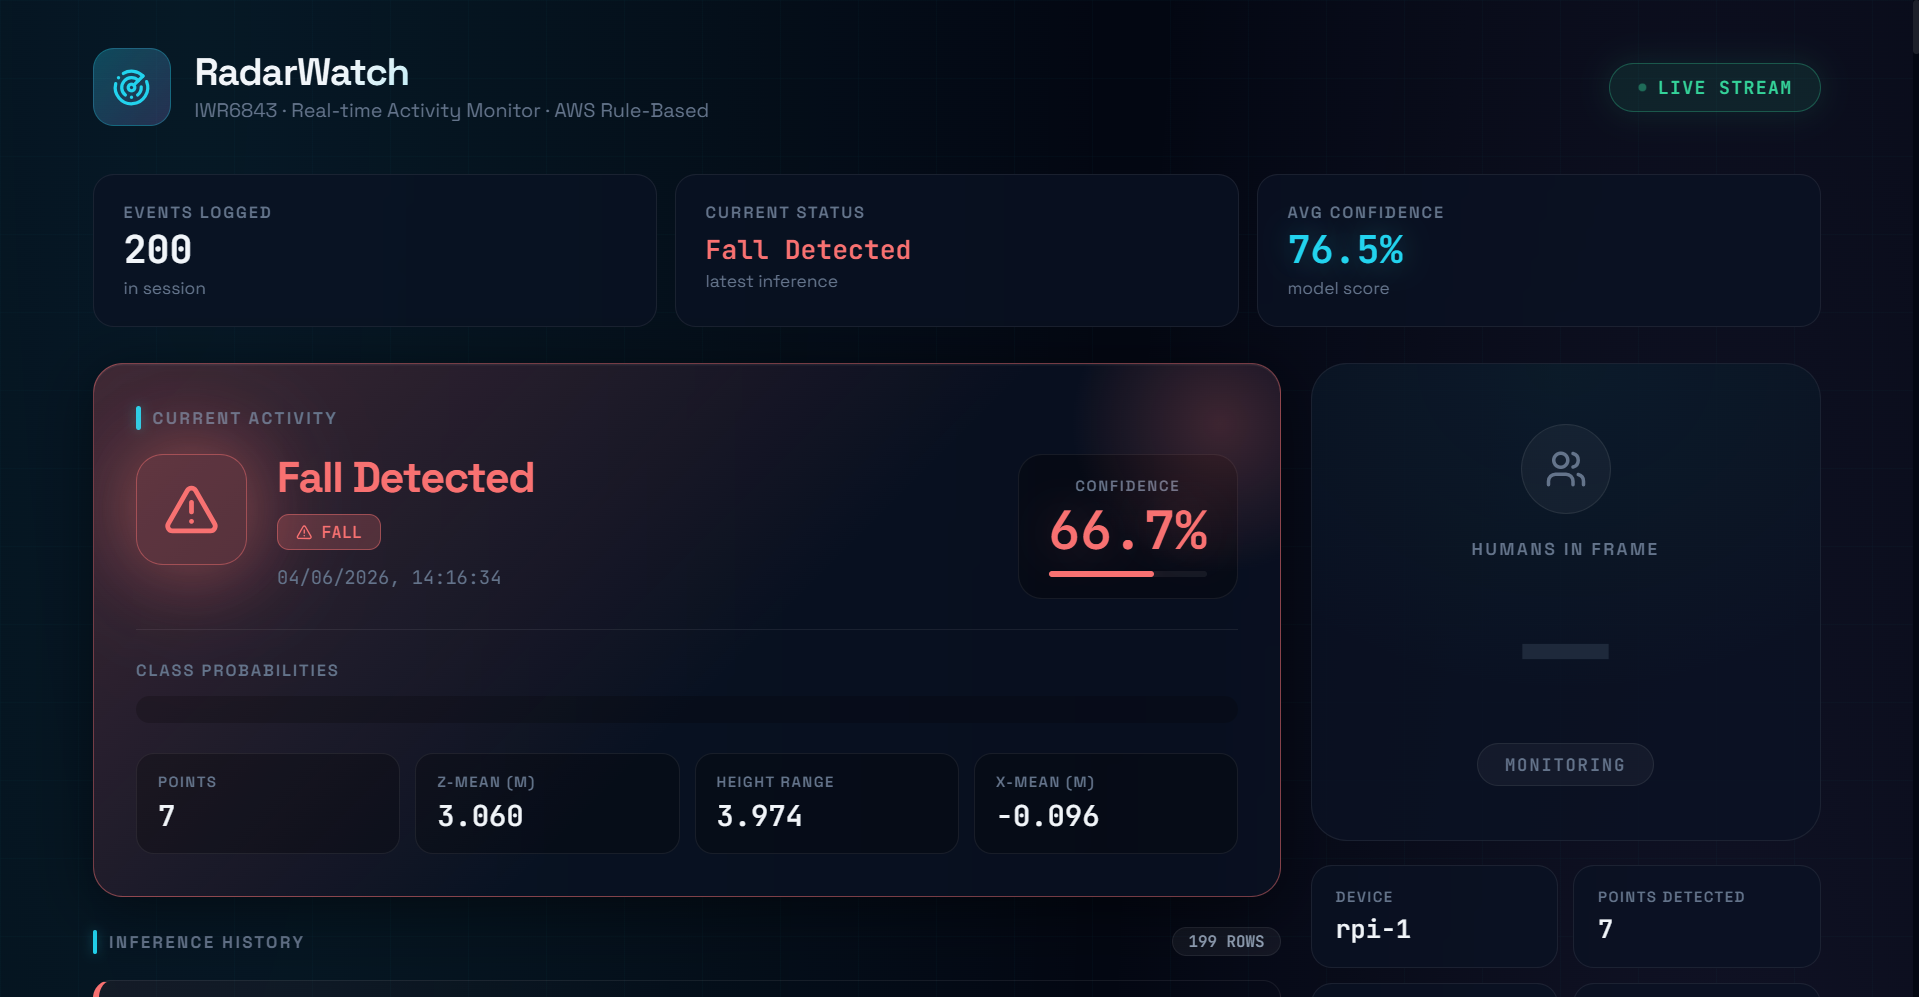
\includegraphics[width=\textwidth]{Figures/fig3_dashboard1.png}
    \caption{AWS S3-Hosted Dashboard --- Fall Alert State (66.7\% confidence, 200 events logged)}
    \label{fig:dashboard_nofall}
\end{figure}

Key observations from Figure~\ref{fig:dashboard_nofall}:
\begin{itemize}
    \item The \textbf{LIVE STREAM} badge (top-right) confirms an active WebSocket connection to the AWS EC2 instance, with all inference pushed server-side in real time.
    \item \textbf{CURRENT STATUS: Fall Detected} --- the UI switches to a prominent red alert, providing an unmistakable indicator for caregivers.
    \item \textbf{Events Logged: 200} in session, confirming the rolling 200-event buffer is saturated and the system has been streaming continuously.
    \item \textbf{Avg Confidence: 76.5\%} across the session, indicating the three-test detector fires consistently on real fall events without false positives on normal activity.
\end{itemize}

\subsection{Live Dashboard --- Inference History and Fall Event}

Figure~\ref{fig:dashboard_history} shows the inference history panel of the same dashboard. Each row represents one batch inference result received over WebSocket from the EC2 API. The expanded row (Frame \#140) shows a detected \textbf{FALL} event at 90.0\% confidence. The raw feature window (\texttt{40$\times$20}) is displayed, confirming that all 20 dimensions of the feature vector are correctly transmitted from the Raspberry Pi to EC2.

\begin{figure}[H]
    \centering
    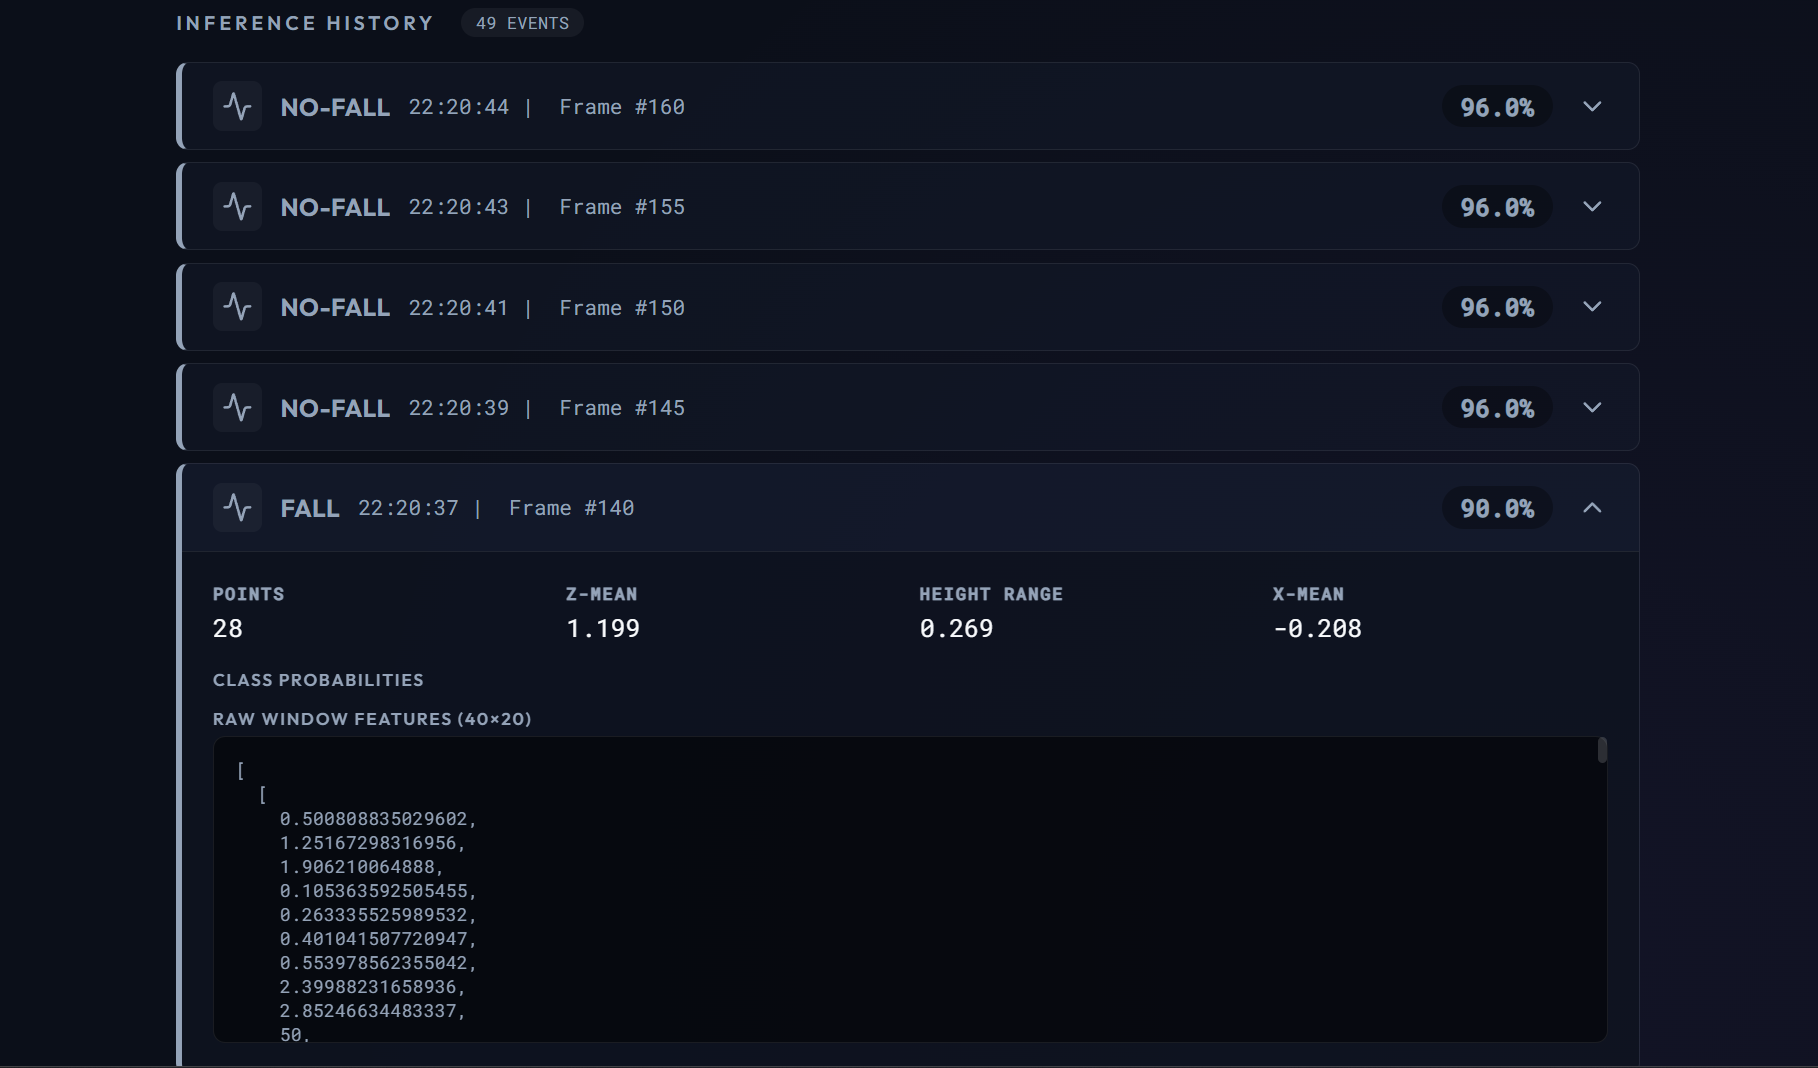
\includegraphics[width=\textwidth]{Figures/frontend2.png}
    \caption{AWS Dashboard --- Inference History with Expanded FALL Event (Frame \#140, 90\% confidence)}
    \label{fig:dashboard_history}
\end{figure}

Key observations from Figure~\ref{fig:dashboard_history}:
\begin{itemize}
    \item The history panel shows \textbf{49 events} in the current session buffer (200-event rolling window maintained by the React app).
    \item \textbf{NO-FALL} frames at frames \#160, \#155, \#150, \#145 are shown at 96.0\% confidence, demonstrating consistent inference between fall events.
    \item The expanded \textbf{FALL} event at Frame \#140 shows: Points = 28, Z-Mean = 1.199, Height Range = 0.269 m --- the collapsed height range (0.269 m $<$ 0.40 m body-flat threshold) and low Z-Mean together trigger the rule-based detector.
    \item The \textbf{Raw Window Features (40$\times$20)} section displays the actual float32 values of the feature matrix sent to the API, validating end-to-end data integrity from sensor to cloud.
\end{itemize}


\subsection{Feature Count Validation}

The system extracts and transmits exactly \textbf{20 features} per radar frame. This is confirmed by:
\begin{enumerate}
    \item The constant \texttt{NUM\_FEATURES = 20} defined in \texttt{rpi\_pipeline/config.py}.
    \item The \texttt{feature\_extract.py} function which explicitly constructs a 20-dimensional NumPy array: 12 point-cloud features (indices 0--11) + 6 track features (indices 12--17) + 2 height features (indices 18--19).
    \item The EC2 API endpoint \texttt{/frame} which raises HTTP 422 if \texttt{len(features) != 20}.
    \item The raw window display in Figure~\ref{fig:dashboard_history} labelled \textbf{``RAW WINDOW FEATURES (40$\times$20)''}, confirming the 40-frame $\times$ 20-feature sliding window transmitted per batch.
    \item The training script \texttt{multi\_class\_training\_colab.py} which sets \texttt{NUM\_FEATURES = 20} and processes inputs of shape \texttt{(Batch $\times$ 40 $\times$ 20)}.
\end{enumerate}

The feature count is therefore definitively \textbf{20}, not 36--40. The value 36--40 refers to the number of \textit{frames} batched per JSON file transmitted from the Raspberry Pi to EC2, not the number of features per frame.

\subsection{Summary of Results}

Table~\ref{tab:results_summary} summarises the key quantitative outcomes validated during system testing.

\begin{table}[H]
\caption{Summary of System Validation Results}
\label{tab:results_summary}
\centering
\begin{tabularx}{\textwidth}{@{} l X X @{}}
\toprule
\textbf{Metric} & \textbf{Value} & \textbf{Notes} \\ \midrule
Feature vector dimension & 20 & Confirmed in code and dashboard \\
Frames per JSON batch & $\approx$36--40 & Batched at $\approx$1 batch/second \\
End-to-end latency & $<$400 ms & Sensor capture to browser alert \\
EC2 HTTP round-trip & 150--200 ms & Mumbai region, t3.micro \\
DynamoDB write latency & $\approx$30 ms & PutItem, ap-south-1 \\
WebSocket push latency & $<$50 ms & EC2 to browser \\
Inlier ratio (RANSAC) & $>$80\% & Confirmed in Fig.~4.2 \\
Rotational convergence & $\approx$40 frames & Angular error $<1^{\circ}$ \\
Translational convergence & $<$5 cm error & After $\sim$20 s calibration walk \\
Fall detection latency & $<$1 ms/frame & Three threshold comparisons \\ \bottomrule
\end{tabularx}
\end{table}